\documentclass{standalone}
\usepackage{tikz}
\usetikzlibrary{patterns, positioning}


\begin{document}
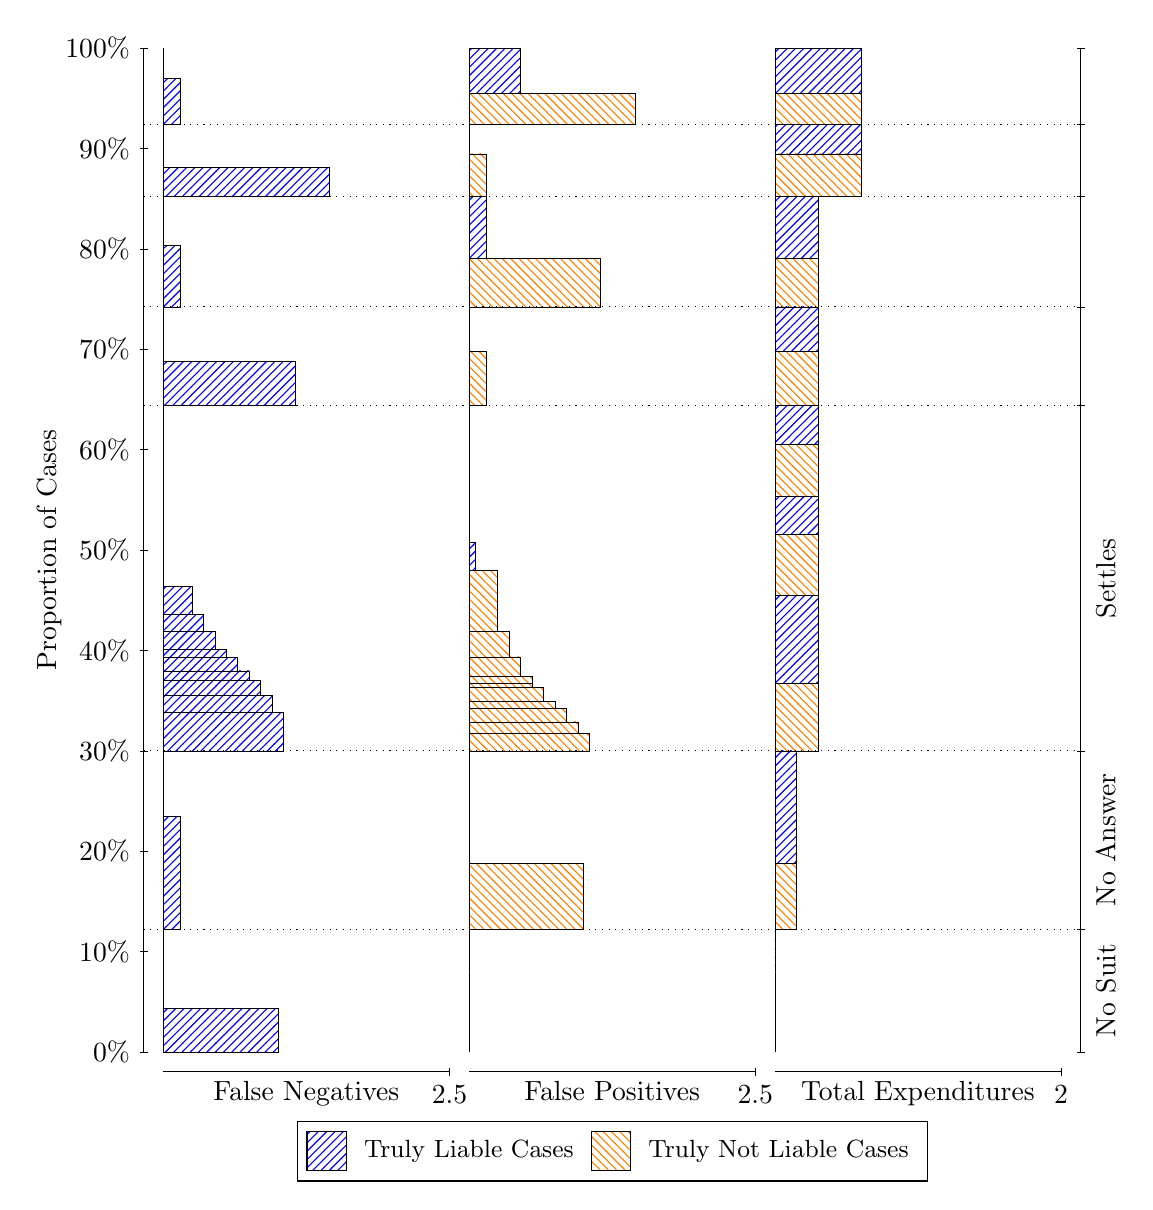
\begin{tikzpicture}
\draw[black, very thin] (1.5,1.75) -- (1.5,14.5);
\node[rotate=90, text=black, anchor=center] at (0.3, 8.125) {Proportion of Cases};
\draw[black, very thin] (1.45,1.75) -- (1.55,1.75);
\node[text=black, anchor=east] at (1.45, 1.75) {0\%};
\draw[black, very thin] (1.45,3.025) -- (1.55,3.025);
\node[text=black, anchor=east] at (1.45, 3.025) {10\%};
\draw[black, very thin] (1.45,4.3) -- (1.55,4.3);
\node[text=black, anchor=east] at (1.45, 4.3) {20\%};
\draw[black, very thin] (1.45,5.575) -- (1.55,5.575);
\node[text=black, anchor=east] at (1.45, 5.575) {30\%};
\draw[black, very thin] (1.45,6.85) -- (1.55,6.85);
\node[text=black, anchor=east] at (1.45, 6.85) {40\%};
\draw[black, very thin] (1.45,8.125) -- (1.55,8.125);
\node[text=black, anchor=east] at (1.45, 8.125) {50\%};
\draw[black, very thin] (1.45,9.4) -- (1.55,9.4);
\node[text=black, anchor=east] at (1.45, 9.4) {60\%};
\draw[black, very thin] (1.45,10.675) -- (1.55,10.675);
\node[text=black, anchor=east] at (1.45, 10.675) {70\%};
\draw[black, very thin] (1.45,11.95) -- (1.55,11.95);
\node[text=black, anchor=east] at (1.45, 11.95) {80\%};
\draw[black, very thin] (1.45,13.225) -- (1.55,13.225);
\node[text=black, anchor=east] at (1.45, 13.225) {90\%};
\draw[black, very thin] (1.45,14.5) -- (1.55,14.5);
\node[text=black, anchor=east] at (1.45, 14.5) {100\%};

\draw[black, very thin] (13.4,1.75) -- (13.4,14.5);
\draw[black, very thin] (13.35,1.75) -- (13.45,1.75);
\node[anchor=west] at (13.35, 1.75) {};
\draw[black, very thin] (13.35,3.3085) -- (13.45,3.3085);
\node[anchor=west] at (13.35, 3.3085) {};
\draw[black, very thin] (13.35,5.5739) -- (13.45,5.5739);
\node[anchor=west] at (13.35, 5.5739) {};
\draw[black, very thin] (13.35,9.9594) -- (13.45,9.9594);
\node[anchor=west] at (13.35, 9.9594) {};
\draw[black, very thin] (13.35,11.213) -- (13.45,11.213);
\node[anchor=west] at (13.35, 11.213) {};
\draw[black, very thin] (13.35,12.614) -- (13.45,12.614);
\node[anchor=west] at (13.35, 12.614) {};
\draw[black, very thin] (13.35,13.528) -- (13.45,13.528);
\node[anchor=west] at (13.35, 13.528) {};
\draw[black, very thin] (13.35,14.5) -- (13.45,14.5);
\node[anchor=west] at (13.35, 14.5) {};

\draw[black, very thin, pattern color=blue, pattern=north east lines] (1.75,1.75) rectangle (3.2033,2.2992);
\draw[black, very thin, pattern color=orange, pattern=north west lines] (1.75,2.2992) rectangle (1.75,3.3085);
\draw[black, very thin, pattern color=blue, pattern=north east lines] (1.75,3.3085) rectangle (1.968,4.7413);
\draw[black, very thin, pattern color=orange, pattern=north west lines] (1.75,4.7413) rectangle (1.75,5.5739);
\draw[black, very thin, pattern color=blue, pattern=north east lines] (1.75,5.5739) rectangle (3.276,6.0582);
\draw[black, very thin, pattern color=blue, pattern=north east lines] (1.75,6.0582) rectangle (3.1307,6.2773);
\draw[black, very thin, pattern color=blue, pattern=north east lines] (1.75,6.2773) rectangle (2.9853,6.4656);
\draw[black, very thin, pattern color=blue, pattern=north east lines] (1.75,6.4656) rectangle (2.84,6.5895);
\draw[black, very thin, pattern color=blue, pattern=north east lines] (1.75,6.5895) rectangle (2.6947,6.7616);
\draw[black, very thin, pattern color=blue, pattern=north east lines] (1.75,6.7616) rectangle (2.5493,6.8594);
\draw[black, very thin, pattern color=blue, pattern=north east lines] (1.75,6.8594) rectangle (2.404,7.0951);
\draw[black, very thin, pattern color=blue, pattern=north east lines] (1.75,7.0951) rectangle (2.2587,7.3083);
\draw[black, very thin, pattern color=blue, pattern=north east lines] (1.75,7.3083) rectangle (2.1133,7.6671);
\draw[black, very thin, pattern color=orange, pattern=north west lines] (1.75,7.6671) rectangle (1.75,9.9594);
\draw[black, very thin, pattern color=blue, pattern=north east lines] (1.75,9.9594) rectangle (3.4213,10.522);
\draw[black, very thin, pattern color=orange, pattern=north west lines] (1.75,10.522) rectangle (1.75,11.213);
\draw[black, very thin, pattern color=blue, pattern=north east lines] (1.75,11.213) rectangle (1.968,11.997);
\draw[black, very thin, pattern color=orange, pattern=north west lines] (1.75,11.997) rectangle (1.75,12.614);
\draw[black, very thin, pattern color=blue, pattern=north east lines] (1.75,12.614) rectangle (3.8573,12.986);
\draw[black, very thin, pattern color=orange, pattern=north west lines] (1.75,12.986) rectangle (1.75,13.528);
\draw[black, very thin, pattern color=blue, pattern=north east lines] (1.75,13.528) rectangle (1.968,14.11);
\draw[black, very thin, pattern color=orange, pattern=north west lines] (1.75,14.11) rectangle (1.75,14.5);
\draw[black, very thin, pattern color=orange, pattern=north west lines] (5.6333,1.75) rectangle (5.6333,2.7592);
\draw[black, very thin, pattern color=blue, pattern=north east lines] (5.6333,2.7592) rectangle (5.6333,3.3085);
\draw[black, very thin, pattern color=orange, pattern=north west lines] (5.6333,3.3085) rectangle (7.0867,4.141);
\draw[black, very thin, pattern color=blue, pattern=north east lines] (5.6333,4.141) rectangle (5.6333,5.5739);
\draw[black, very thin, pattern color=orange, pattern=north west lines] (5.6333,5.5739) rectangle (7.1593,5.795);
\draw[black, very thin, pattern color=orange, pattern=north west lines] (5.6333,5.795) rectangle (7.014,5.9421);
\draw[black, very thin, pattern color=orange, pattern=north west lines] (5.6333,5.9421) rectangle (6.8687,6.1141);
\draw[black, very thin, pattern color=orange, pattern=north west lines] (5.6333,6.1141) rectangle (6.7233,6.2039);
\draw[black, very thin, pattern color=orange, pattern=north west lines] (5.6333,6.2039) rectangle (6.578,6.3792);
\draw[black, very thin, pattern color=orange, pattern=north west lines] (5.6333,6.3792) rectangle (6.4327,6.4266);
\draw[black, very thin, pattern color=orange, pattern=north west lines] (5.6333,6.4266) rectangle (6.4327,6.5156);
\draw[black, very thin, pattern color=orange, pattern=north west lines] (5.6333,6.5156) rectangle (6.2873,6.7679);
\draw[black, very thin, pattern color=orange, pattern=north west lines] (5.6333,6.7679) rectangle (6.142,7.0939);
\draw[black, very thin, pattern color=orange, pattern=north west lines] (5.6333,7.0939) rectangle (5.9967,7.8661);
\draw[black, very thin, pattern color=blue, pattern=north east lines] (5.6333,7.8661) rectangle (5.706,8.2249);
\draw[black, very thin, pattern color=blue, pattern=north east lines] (5.6333,8.2249) rectangle (5.6333,9.9594);
\draw[black, very thin, pattern color=orange, pattern=north west lines] (5.6333,9.9594) rectangle (5.8513,10.651);
\draw[black, very thin, pattern color=blue, pattern=north east lines] (5.6333,10.651) rectangle (5.6333,11.213);
\draw[black, very thin, pattern color=orange, pattern=north west lines] (5.6333,11.213) rectangle (7.3047,11.83);
\draw[black, very thin, pattern color=blue, pattern=north east lines] (5.6333,11.83) rectangle (5.8513,12.614);
\draw[black, very thin, pattern color=orange, pattern=north west lines] (5.6333,12.614) rectangle (5.8513,13.156);
\draw[black, very thin, pattern color=blue, pattern=north east lines] (5.6333,13.156) rectangle (5.6333,13.528);
\draw[black, very thin, pattern color=orange, pattern=north west lines] (5.6333,13.528) rectangle (7.7407,13.919);
\draw[black, very thin, pattern color=blue, pattern=north east lines] (5.6333,13.919) rectangle (6.2873,14.5);
\draw[black, very thin, pattern color=orange, pattern=north west lines] (9.5167,1.75) rectangle (9.5167,2.7592);
\draw[black, very thin, pattern color=blue, pattern=north east lines] (9.5167,2.7592) rectangle (9.5167,3.3085);
\draw[black, very thin, pattern color=orange, pattern=north west lines] (9.5167,3.3085) rectangle (9.7892,4.141);
\draw[black, very thin, pattern color=blue, pattern=north east lines] (9.5167,4.141) rectangle (9.7892,5.5739);
\draw[black, very thin, pattern color=orange, pattern=north west lines] (9.5167,5.5739) rectangle (10.062,6.4266);
\draw[black, very thin, pattern color=blue, pattern=north east lines] (9.5167,6.4266) rectangle (10.062,7.5462);
\draw[black, very thin, pattern color=orange, pattern=north west lines] (9.5167,7.5462) rectangle (10.062,8.3184);
\draw[black, very thin, pattern color=blue, pattern=north east lines] (9.5167,8.3184) rectangle (10.062,8.8027);
\draw[black, very thin, pattern color=orange, pattern=north west lines] (9.5167,8.8027) rectangle (10.062,9.4701);
\draw[black, very thin, pattern color=blue, pattern=north east lines] (9.5167,9.4701) rectangle (10.062,9.9594);
\draw[black, very thin, pattern color=orange, pattern=north west lines] (9.5167,9.9594) rectangle (10.062,10.651);
\draw[black, very thin, pattern color=blue, pattern=north east lines] (9.5167,10.651) rectangle (10.062,11.213);
\draw[black, very thin, pattern color=orange, pattern=north west lines] (9.5167,11.213) rectangle (10.062,11.83);
\draw[black, very thin, pattern color=blue, pattern=north east lines] (9.5167,11.83) rectangle (10.062,12.614);
\draw[black, very thin, pattern color=orange, pattern=north west lines] (9.5167,12.614) rectangle (10.607,13.156);
\draw[black, very thin, pattern color=blue, pattern=north east lines] (9.5167,13.156) rectangle (10.607,13.528);
\draw[black, very thin, pattern color=orange, pattern=north west lines] (9.5167,13.528) rectangle (10.607,13.919);
\draw[black, very thin, pattern color=blue, pattern=north east lines] (9.5167,13.919) rectangle (10.607,14.5);
\draw[black, dotted] (1.5,3.3085) -- (13.4,3.3085);
\draw[black, dotted] (1.5,5.5739) -- (13.4,5.5739);
\draw[black, dotted] (1.5,9.9594) -- (13.4,9.9594);
\draw[black, dotted] (1.5,11.213) -- (13.4,11.213);
\draw[black, dotted] (1.5,12.614) -- (13.4,12.614);
\draw[black, dotted] (1.5,13.528) -- (13.4,13.528);
\draw[black, very thin] (1.75,1.5) -- (5.3833,1.5);
\node[text=black, anchor=north] at (3.5667, 1.5) {False Negatives};
\draw[black, very thin] (5.3833,1.45) -- (5.3833,1.55);
\node[text=black, anchor=north] at (5.3833, 1.45) {2.5};

\draw[black, very thin] (5.6333,1.5) -- (9.2667,1.5);
\node[text=black, anchor=north] at (7.45, 1.5) {False Positives};
\draw[black, very thin] (9.2667,1.45) -- (9.2667,1.55);
\node[text=black, anchor=north] at (9.2667, 1.45) {2.5};

\draw[black, very thin] (9.5167,1.5) -- (13.15,1.5);
\node[text=black, anchor=north] at (11.333, 1.5) {Total Expenditures};
\draw[black, very thin] (13.15,1.45) -- (13.15,1.55);
\node[text=black, anchor=north] at (13.15, 1.45) {2};

\node[text=black, centered, rotate=90] at (13.72, 2.5292) {No Suit};
\node[text=black, centered, rotate=90] at (13.72, 4.4412) {No Answer};
\node[text=black, centered, rotate=90] at (13.72, 7.7666) {Settles};





\draw (7.449999999999999,1.5) node[draw=none] (baseCoordinate) {};
\begin{scope}[align=center]
        \matrix[scale=0.5, draw=black, below=0.5cm of baseCoordinate, nodes={draw}, column sep=0.1cm]{
            \node[rectangle, draw, minimum width=0.5cm, minimum height=0.5cm, pattern color=blue, pattern=north east lines] {}; &
            \node[draw=none, font=\small, text=black] (B) {Truly Liable Cases}; &
            \node[rectangle, draw, minimum width=0.5cm, minimum height=0.5cm, pattern color=orange, pattern=north west lines] {}; &
            \node[draw=none, font=\small, text=black] (B) {Truly Not Liable Cases}; \\
            };
\end{scope}

\end{tikzpicture}
\end{document}